\documentclass{beamer}

\usepackage{préambule}

\title{Activité : partage de téléphones}
\author{}
\date{}

\begin{document}

\begin{frame}
	\maketitle
\end{frame}

\begin{frame}
	Un groupe de 24 personnes possèdent chacune 0, 1 ou plus téléphones portables. \vspace{1em}

	\uline{Si chaque personne avait autant de téléphones}, combien chacun en aurait-il ?
\end{frame}

\begin{frame}
	\begin{center}
		\begin{tabular}{|l|c|c|c|c|c|c|c|}
			\hline
			Nombre de téléphones & 0 & 1 & 2 & 3 & 4 & 5 & 6
			\\ \hline
			Effectif             & 8 & 9 & 0 & 5 & 1 & 1 & 0
			\\ \hline
		\end{tabular}
	\end{center}
\end{frame}

\begin{frame}
	\begin{center}
		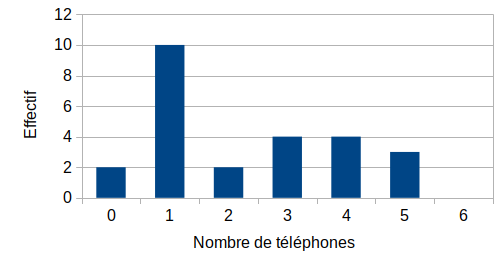
\includegraphics[width=\textwidth]{Images/Diagramme en barres.png}
	\end{center}
\end{frame}

\begin{frame}
	\begin{center}
		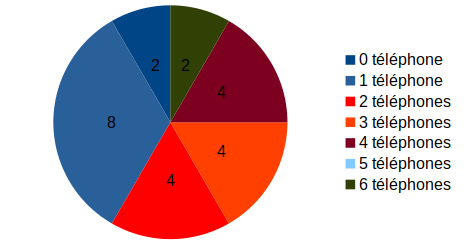
\includegraphics[width=\textwidth]{Images/Diagramme circulaire.png}
	\end{center}
\end{frame}

\end{document}